\documentclass[8pt,a4paper]{article}

%\usepackage[latin1]{inputenc}
\usepackage{german}
\usepackage{a4wide}
\usepackage{url}
\usepackage{graphicx}

%\usepackage[    
%%    style=authoryear,   
%    natbib=true,     
%    firstinits=true,
%    sorting=ydnt,
%    defernumbers,
%    maxnames=50
%]{biblatex}
%\addbibresource{CV_Abesser_Publications.bib}

\renewcommand{\refname}{Books, Book Chapters, Articles}

\parindent 0cm
%\oddsidemargin 0.04cm
\topmargin -1.5cm
\oddsidemargin -1cm
\textwidth 17cm
\textheight 30cm

\newenvironment{itemizePacked}{
\begin{itemize}
  \setlength{\itemsep}{1pt}
  \setlength{\parskip}{3pt}
  \setlength{\parsep}{0pt}
  \renewcommand{\labelitemi}{$\bullet$}
}{\end{itemize}}

\newenvironment{itemizePacked2}{
\begin{itemize}
  \setlength{\itemsep}{1pt}
  \setlength{\parskip}{0pt}
  \setlength{\parsep}{0pt}
  \renewcommand{\labelitemi}{$-$}
}{\end{itemize}}

\begin{document}

\pagestyle{empty}

\vspace{1cm}
%\begin{center}
%\begin{center}
%{\LARGE\bf Chronologischer Lebenslauf}
\begin{minipage}{13.5cm}
\vspace{-5.0cm}
{\large\bf Curriculum Vitae}
\end{minipage}
\begin{minipage}{3.5cm}
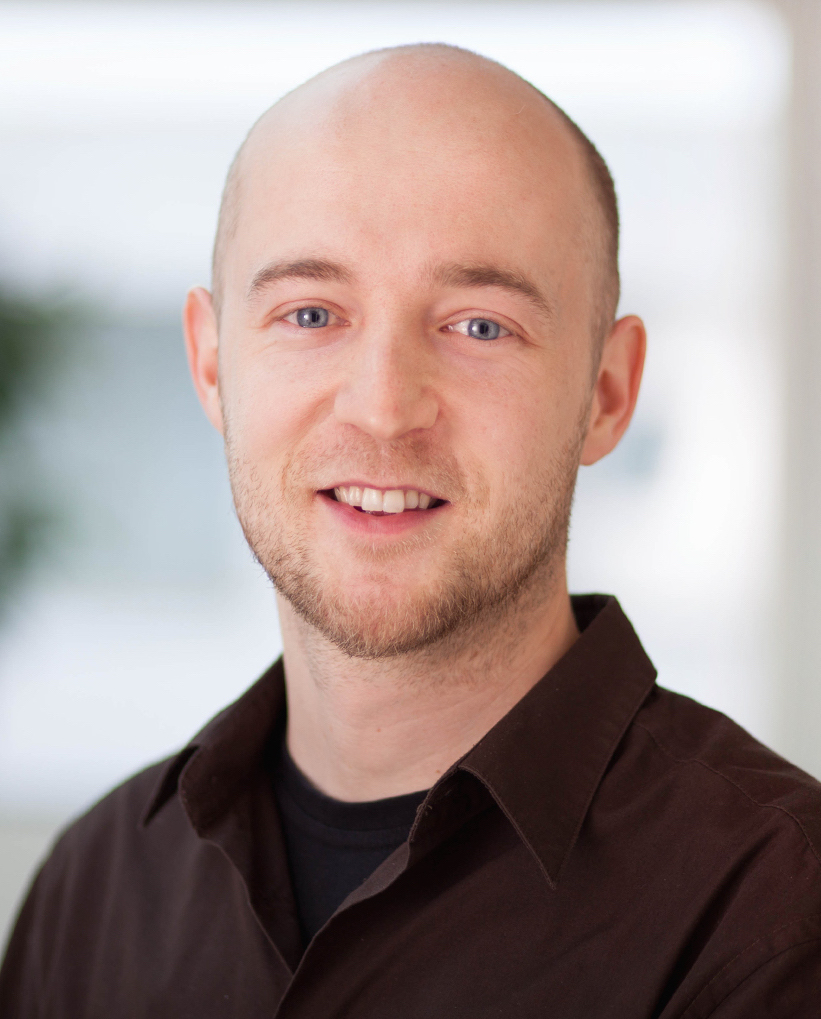
\includegraphics[width=3.5cm]{CV_Abesser_Foto}
\end{minipage}
%\end{center}

\vspace{-3.5cm}

\begin{tabular}{p{3.1cm}p{12cm}}
{\bf Name:} &   {\bf Dr. Jakob Abe{\ss}er}\\
{\bf Address:}  & Annemarie-Becker-Stra{\ss}e 16, D-99092 Erfurt\\
                  & Tel.: 0176-61104420 (pr.), 03677-467288\\
                  & Email: jakob.abesser@idmt.fraunhofer.de \\
                  & \scriptsize http://www.idmt.fraunhofer.de/en/institute/doctorands/abesser.html  \\
                  & \scriptsize https://jakobabesser.github.io/ \normalsize \\
{\bf Birth date/place:}  & 03.\ May 1983 / Jena \\
{\bf Family status:}   & Married, two children  \\
{\bf Citizenship:}   & German \\
\end{tabular}

%\bigskip
\vspace*{1.0cm}


\begin{tabular}{p{3.1cm}p{3.0cm}p{10cm}}
{\bf Recent Positions:}  
& since 2020  & Senior Scientist, Fraunhofer IDMT, Ilmenau, Germany \\

& since 2018 & Principal Investigator (DFG-funded project ``Informed Sound Activity Detection in Music Recordings (ISAD)'' \\

& 2014 -- 2018 & Postdoctoral Researcher, Semantic Music Technologies, Fraunhofer IDMT, Ilmenau, Germany \\
{\bf } & 2012 -- 2017 &	Wissenschaftlicher Mitarbeiter / Postdoctoral Researcher, Jazzomat Research Project, University of Music Franz Liszt, Weimar, Germany\\
{\bf } & 2008 -- 2014 &	Wissenschaftlicher Mitarbeiter, Semantic Music Technologies, Fraunhofer Institute for Digital Media Technologies (IDMT), Ilmenau, Germany \bigskip\\
%
{\bf Education:}  
{\bf } & 2014 &	Ph.D., Media Technology, Technische Universit{\"a}t Ilmenau\\
{\bf } & 2008 &	Diplom, Computer Engineering (Ingenieurinformatik), Technische Universit{\"a}t Ilmenau\\
{\bf } & 2001 &	Abitur, Goetheschule Ilmenau \bigskip\\
%
{\bf Research Stays \& Study Programs:}&
 05/2010 - 08/2010 & Doctoral research stay, Finnish Centre of Excellence in Interdisciplinary Music Research, University of Jyv{\"a}skyl{\"a}, Finnland (DAAD scholarship ``Kurzzeitstipendium f{\"u}r Doktoranden)\\
{\bf } & 09/2005 -- 02/2006 & Computer science study at Universit{\'e} Paul Verlain, Metz, France (ERASMUS scholarship)\\
\bigskip\\
%
{\bf Research Areas:}& 
{\bf } & Machine Listening, Music Information Retrieval, Audio Signal Processing, Machine Learning, Deep Learning
\end{tabular}

\pagebreak[4]\clearpage
%\vspace*{0.2cm}

{\bf Scientific Activities \& Projects (Selection):}
\begin{itemizePacked}
\item Member of the International Society for Music Information Retrieval %(since ??) %(since October 2009)
\item BMBF-funded project: GlobalMusic2one (2008-2011): Adaptive, hybride Suchtechnologien f{\"u}r Globale Musikbest{\"a}nde
\item BMBF-funded project: SyncGlobal (2012-2013): Globale Musiksuche zur cross-modalen Synchronisation mit Videoinhalten
\item DFG-Project (2018-2021): Informed Sound Activity Detection in Music Recordings (ISAD) 
\item DFG-Project (2012-2017): Melodisch-rhythmische Gestaltung von Jazzimprovisationen. Rechnerbasierte Musikanalyse einstimmiger Jazzsoli
\item DFG-Project (2010-2013): Entwicklung und empirische Validierung eines Modells musikpraktischer Kompetenzen (Kopra-M)

\end{itemizePacked}

\vspace*{0.2cm}

{\bf Awards \& Honors:}
\begin{itemizePacked}
\item 2019: Best paper award (14th International Symposium on Computer Music Multidisciplinary Research) with Matthias Nowakowski and Christof Wei\ss
\item 2010: DAAD scholarship ``Kurzzeitstipendium f{\"u}r Doktoranden''
\item 2005-2006: ERASMUS scholarship
\end{itemizePacked}

\vspace*{0.2cm}

\nocite{Abesser:2020:AS}
\nocite{Pfleiderer:2017:BOOK}
\nocite{Abesser_2017_IEEE_b}
\nocite{Abesser:2017:IEEE}
\nocite{Frieler:2016:MS}
\nocite{Abesser:2014:PHD}
\nocite{Abesser:2012:CMMR}
\nocite{Abesser:2012:JNMR}
\nocite{Dittmar:2012:MMP}
\nocite{Brandenburg:2009:BOOK}


\bibliographystyle{IEEEtranS}
\bibliography{CV_Abesser_Publications}

For a full list see: \url{https://jakobabesser.github.io/publications.html}

\vspace{1cm}

Erfurt, November 2020
\end{document}



